\subsubsection{MULTI-SCALE 3D INTERPRETATION}
To understand this technique we need to analyze the same target in 
two different positions, as in Fig. \ref{fig:multiscale3d}.

\begin{figure}[H]
\centering
  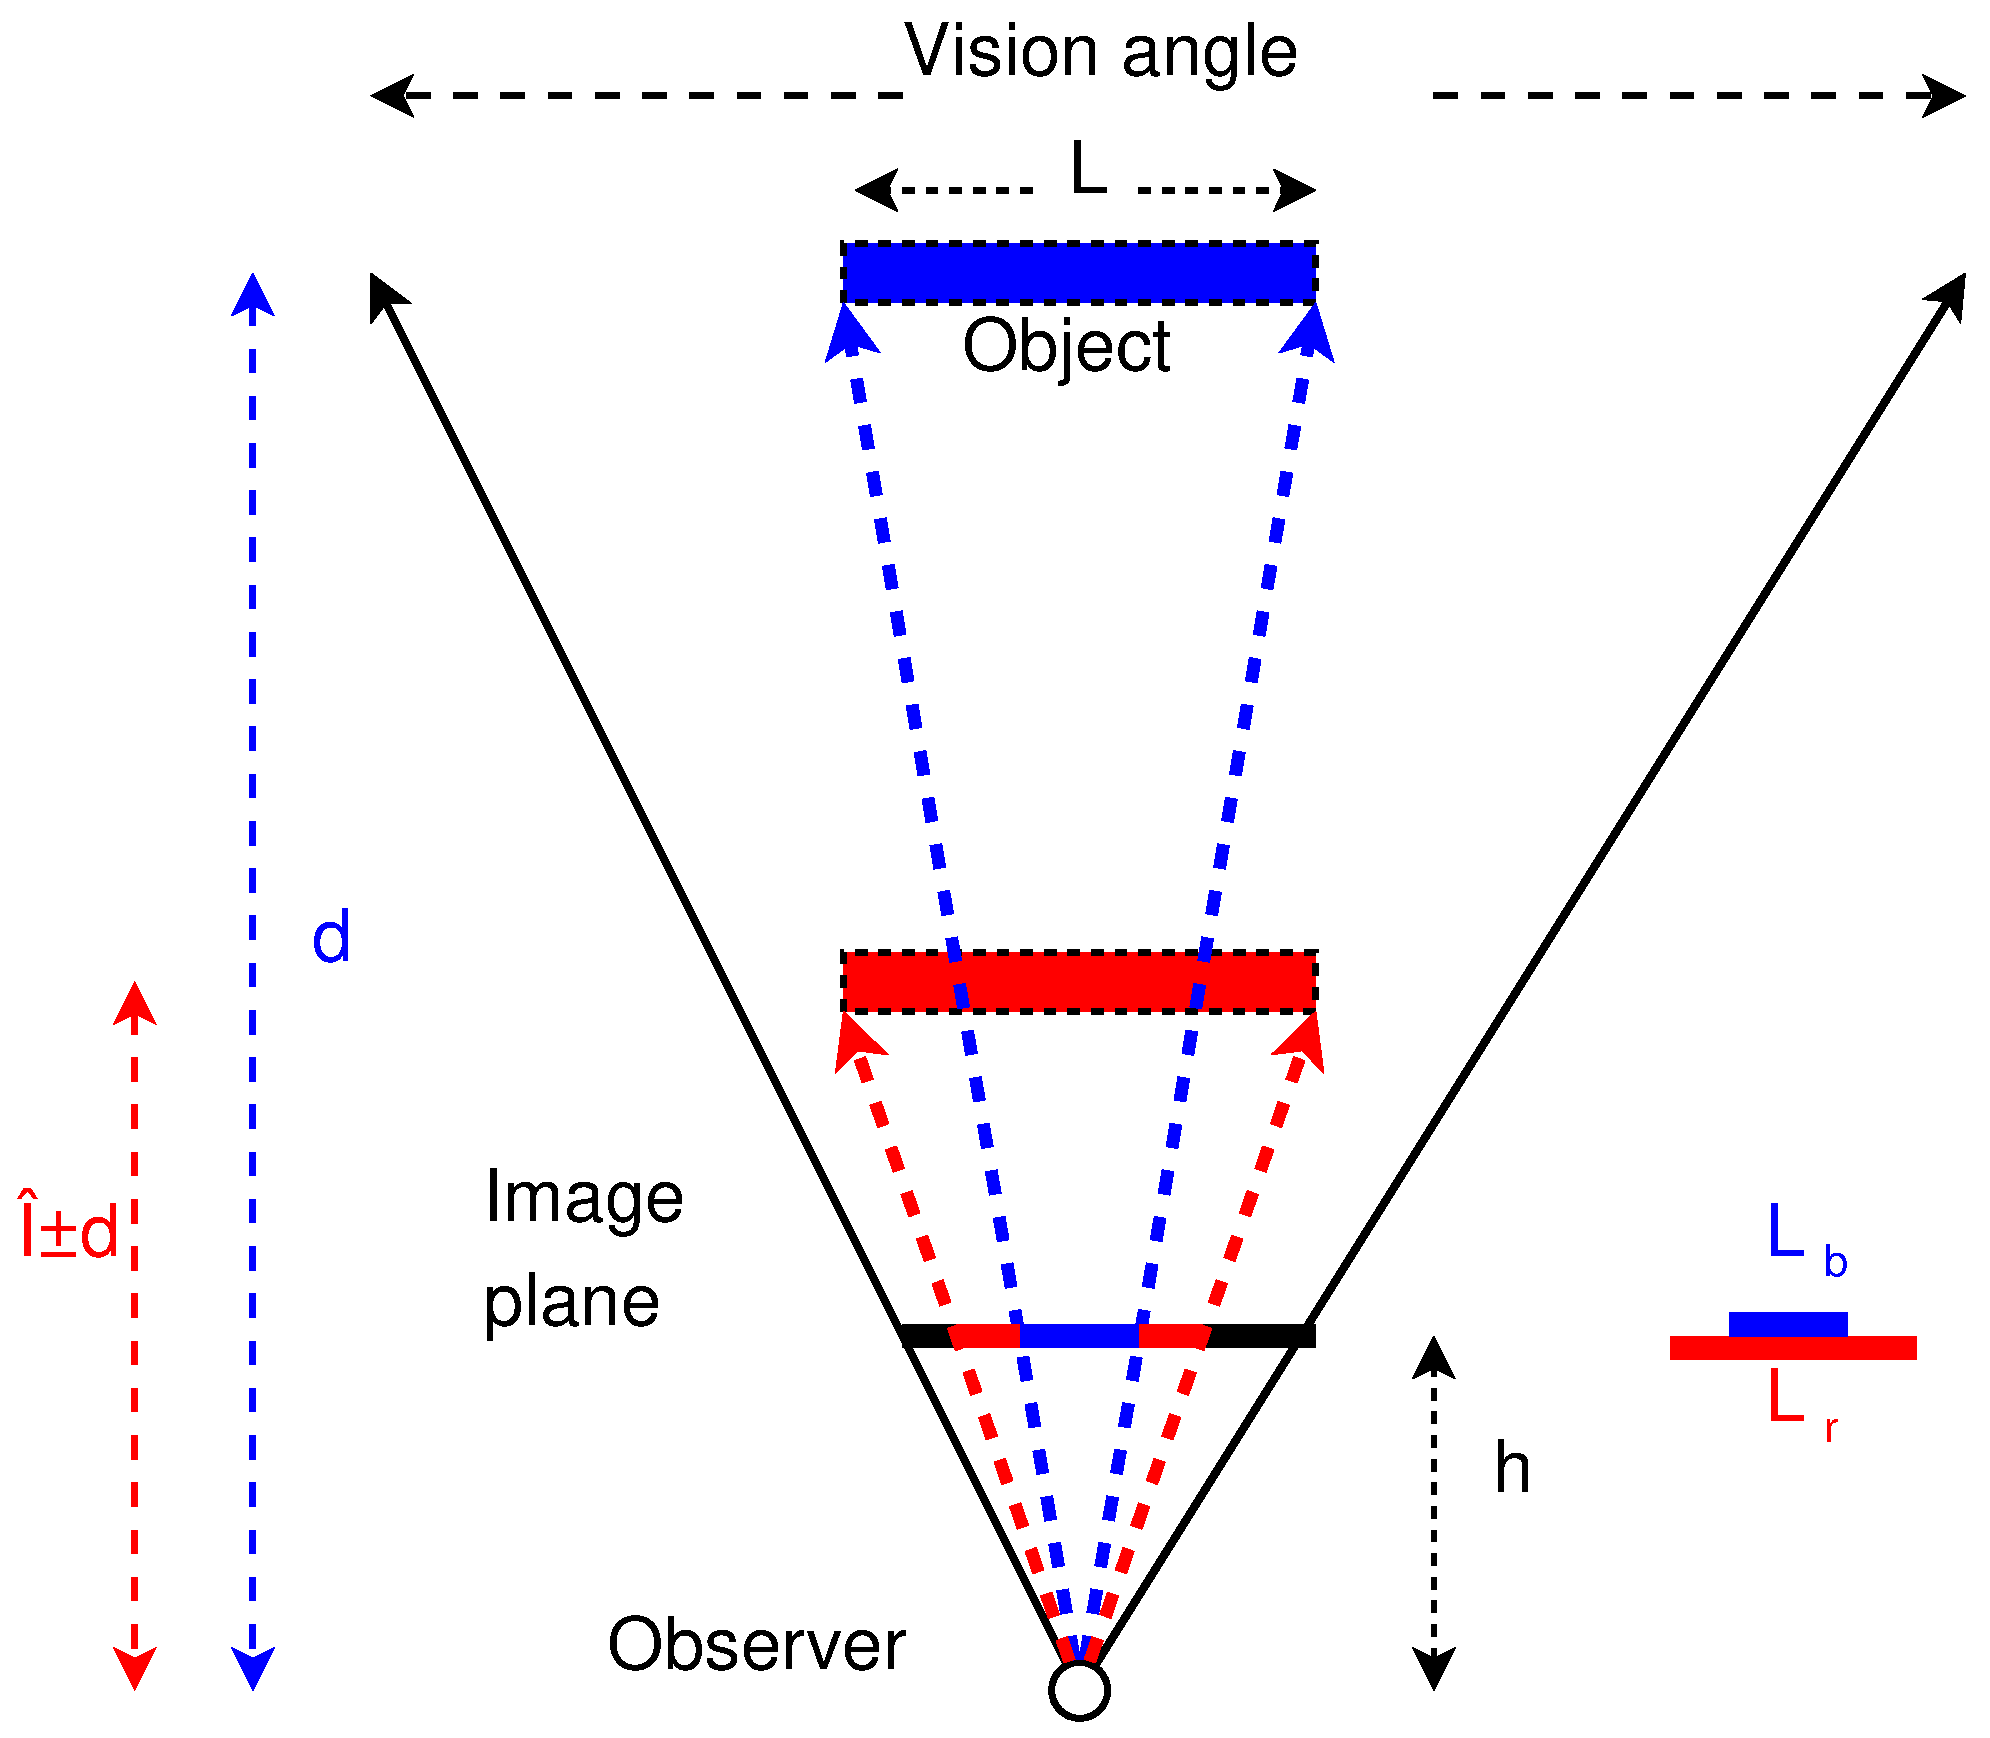
\includegraphics[width=.7\columnwidth]{images/Diagrama3.eps}
  \caption{The multi-scale tracking.}
  \label{fig:multiscale3d}
\end{figure}
Fig. 3 shows the same target at two different distances $d$ and $\alpha d$, in blue and red respectively.
The image plane is located at a distance $h$ of the observer.
The projections of target, in blue and red, in the image plane are
$L_b$ and $L_r$, respectively. Making a simple inspection in the
formed triangles, we can see that $\frac{h}{d}=\frac{L_b}{L}$ and 
$\frac{h}{\alpha d}=\frac{L_r}{L}$, and consequently $L_b/\alpha= L_r$. 
From the point of view of the observer, this implies that if a target 
is located at a distance $d$ in the time $t_0$,  and at a distance $\alpha d$ in the time $t_1$, 
then the width of the target in the image plane is altered by a factor of 1/$\alpha$, 
and consequently its area is altered by a factor of 1/$\alpha^2$.

The algorithm then search targets using different discrete values of $\alpha$,
tracks targets nearest with $\alpha<1$ and targets farthest with $\alpha>1$.

%usa Multi-resolution match criteria e explica isso dos tamanhos

\subsubsection{DEPARTURE FACTOR - RELATIVE VELOCITY}
The departure factor is a dimensionless number related to the rate of approaching 
or departure of a target to the observer. The factor
is determined in (\ref{eq:relarea}),

\begin{equation}\label{eq:relarea}
f_a \equiv \alpha^2 \equiv \frac{Area_r}{Area_f} 
\end{equation}

where $f_a$ and $\alpha$ are defined as area factor and departure factor, 
respectively; $Area_r$ is the ROI area and $Area_f$ 
is the area of the analysis region in the current image. 

Thus, if we consider that the analyzed target  in the $ROI$ was to a distance $d_0$,
them the target in the analysis region will be to a distance $\alpha d_0$ (or $\sqrt{f_a} d_0$);
thus, if the $i-th$ image was analyzed, then $\alpha_i$ and $d_i=\alpha_i d_0$ will be obtained.

The departure factor, $\alpha_i$, has two interpretations: if the rate of departure increase quickly, 
means that the target is departing. If the factor decreases, the 
target is approaching.

The relative velocity is calculate using a simples equation of kinematic in physics:
\begin{equation}
 v_i = \frac{\Delta s}{\Delta t}= \frac{s_i-s_{i-1}}{\Delta t}.
\end{equation}

where the vector $v_i$ represents the relative velocity in the i-th image, 
$s_i=(x_i,y_i,d_i)$ is the position of match in the i-th image
and $\Delta t$ is the sampling time between images.
Additionally, we call of velocity of departure factor, $v^d_i$, to 
the scalar number which represents the depth component
of the vector $v_i$.

The calculated  $v^d_i$ value is relative, for the simple reason that the distance (depth) between the 
camera (observer) and the target in the instant i-th will be referenced to $d_0$, 
given that the distance of the initial $ROI$ is established by definition to 1.
Finally, in all cases, the position $s_i$ is relative to the observer (a moving reference system).

